\documentclass[10pt, a5paper]{article}
\usepackage{pdfpages}
\usepackage{parallel}
\usepackage[T2A]{fontenc}
\usepackage{ucs}
\usepackage[utf8x]{inputenc}
\usepackage[polish,english,russian]{babel}
\usepackage{hyperref}
\usepackage{rotating}
\usepackage[inner=2cm,top=1.8cm,outer=2cm,bottom=2.3cm,nohead]{geometry}
\usepackage{listings}
\usepackage{graphicx}
\usepackage{wrapfig}
\usepackage{longtable}
\usepackage{indentfirst}
\usepackage{array}
\newcolumntype{P}[1]{>{\raggedright\arraybackslash}p{#1}}
\frenchspacing
\usepackage{fixltx2e} %text sub- and superscripts
\usepackage{icomma} % коскі ў матэматычным рэжыме
\PreloadUnicodePage{4}

\newcommand{\longpage}{\enlargethispage{\baselineskip}}
\newcommand{\shortpage}{\enlargethispage{-\baselineskip}}

\def\switchlang#1{\expandafter\csname switchlang#1\endcsname}
\def\switchlangbe{
\let\saverefname=\refname%
\def\refname{Літаратура}%
\def\figurename{Іл.}%
}
\def\switchlangen{
\let\saverefname=\refname%
\def\refname{References}%
\def\figurename{Fig.}%
}
\def\switchlangru{
\let\saverefname=\refname%
\let\savefigurename=\figurename%
\def\refname{Литература}%
\def\figurename{Рис.}%
}

\hyphenation{admi-ni-stra-tive}
\hyphenation{ex-pe-ri-ence}
\hyphenation{fle-xi-bi-li-ty}
\hyphenation{Py-thon}
\hyphenation{ma-the-ma-ti-cal}
\hyphenation{re-ported}
\hyphenation{imp-le-menta-tions}
\hyphenation{pro-vides}
\hyphenation{en-gi-neering}
\hyphenation{com-pa-ti-bi-li-ty}
\hyphenation{im-pos-sible}
\hyphenation{desk-top}
\hyphenation{elec-tro-nic}
\hyphenation{com-pa-ny}
\hyphenation{de-ve-lop-ment}
\hyphenation{de-ve-loping}
\hyphenation{de-ve-lop}
\hyphenation{da-ta-ba-se}
\hyphenation{plat-forms}
\hyphenation{or-ga-ni-za-tion}
\hyphenation{pro-gramming}
\hyphenation{in-stru-ments}
\hyphenation{Li-nux}
\hyphenation{sour-ce}
\hyphenation{en-vi-ron-ment}
\hyphenation{Te-le-pathy}
\hyphenation{Li-nux-ov-ka}
\hyphenation{Open-BSD}
\hyphenation{Free-BSD}
\hyphenation{men-ti-on-ed}
\hyphenation{app-li-ca-tion}

\def\progref!#1!{\texttt{#1}}
\renewcommand{\arraystretch}{2} %Іначай формулы ў матрыцы зліпаюцца з лініямі
\usepackage{array}

\def\interview #1 (#2), #3, #4, #5\par{

\section[#1, #3, #4]{#1 -- #3, #4}
\def\qname{LVEE}
\def\aname{#1}
\def\q ##1\par{{\noindent \bf \qname: ##1 }\par}
\def\a{{\noindent \bf \aname: } \def\qname{L}\def\aname{#2}}
}

\def\interview* #1 (#2), #3, #4, #5\par{

\section*{#1\\{\small\rm #3, #4. #5}}

\def\qname{LVEE}
\def\aname{#1}
\def\q ##1\par{{\noindent \bf \qname: ##1 }\par}
\def\a{{\noindent \bf \aname: } \def\qname{L}\def\aname{#2}}
}

\begin{document}
\title{Virtualization"=based illustrated reviews of the software history}
\author{Dmitriy Kostiuk, Pavel Lutsiuk, Sergey Vlasenko, \\ Vitaliy Zheludok "--- Brest, Belarus\footnote{\url{dmitriykostiuk@gmail.com}, \url{http://lvee.org/ru/abstracts/144}}}
\maketitle
\begin{abstract}
Experience of using virtual machines instead of screenshots in a visual timeline of GUI is reviewed. Availability of materials is considered as far as problems of QEMU"=based nested virtualiza\-tion. A solution is proposed for free distribution of F/LOSS virtualized items with a possibility to automatically integrate proprietary ones in case of their presence. 
\end{abstract}
Although technically working with the new information technologies doesn't demands knowing the history of their development, however specialist who formulates or applies modern theory without knowledge of its history, runs the risk of repeating the mistakes of predecessors personally one by one.

In the context of spoken above statement this project lies, providing the user of a local network or a standalone workstation with the set of chronologically HTML documents, each with a description of the specific graphical operating system and its live illustration in the form of built"=in frame with the screen of a running virtual machine (thanks to the performance of today's notebooks and desktop PCs, this task is easy enough). The information content of this project is based on the lecture course on the history of graphical user interface, including 40 desktop and 30 mobile operating systems and desktop environments.

Technical infrastructure implementing such informational materials, is close to one reviewed in \cite{kostiuk1} and includes following components: 
\begin{itemize}
\item QEMU virtual machine with hardware virtualization support,
\item noVNC VNC client, written in JavaScript and HTML5, 
\item JavaScript framework to display informational materials in one interactive timeline.
\end{itemize}

Running the scheme shown on the figure 1 is done by a startup script, which scans subdirectories in search for the information elements: pages with the content, virtual machine images and scripts to run them. Script passes VNC port numbers to discovered virtual machines and reconstructs HTML document to include of pages with information materials into timeline. This component based approach allows to divide the information, making free/libre parts publicly available on the net\-work, and taking away from public access those virtualized systems, which can not be redistributed due to the terms of commercial licenses.

\begin{figure}[h!]
  \centering
  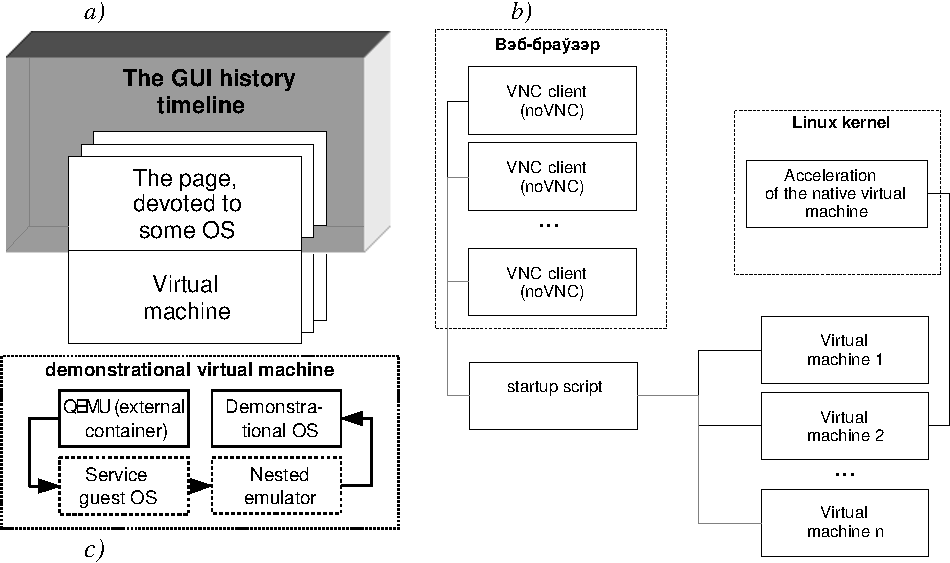
\includegraphics[scale=0.65]{100_2014_w-kostiuk1crop_en}
  \caption{Scheme of the document building (a), and components interaction (b) with nested virtualization (c)}
\end{figure}

The virtual machine is used as a fully isolated container storing a snapshot of the running OS \cite{kostiuk2}. Choice of QEMU is caused by the extremely simple transfer of virtual machine images between computers, and also by its ability to emulate not only x86"=compatible platforms, but also ones based on SPARC, PowerPC, Motorola 68k, MIPS and ARM processors, which are necessary to run many operating systems from 80s and 90s. However, currently multiplatformness of QEMU is poorly used, because the support of peripheral devices on alternative platforms at this emulator is rarely sufficient to boot ancient operating systems.

At the same time, there are emulators available to support virtually all ancient Intel"=incompatible systems "---community"=developed ones or created as the part of commercial SDK. The first variant is more common in desktop operating systems, so it was possible to enrich the timeline with Xerox Alto, Amiga, RiscOS, Apple Lisa, MacOS of 1.x, 7.x and X versions. Proprietary emulators for desktop operating systems are rare case and usually belong to the manufacturer of the OS, as in the case of Xerox GlobalView emulator. In case of mobile operating systems emulators from the SDK are dominating, such as Psion EPOC16 and EPOC32, PalmOS, Magic Cap, Windows CE, pre"=release versions of Android SDK. For now we use only one community"=developed mobile OS emulator "---Open Einstein project, which allows to run NewtonOS.

However, all these emulators don't support snapshots and the VNC protocol. Therefore a large part of demos is build along with the the nested virtualization scheme (see Fig. 1) where QEMU plays the role of an external container. 

Of course many operating systems do not require nested virtualiza\-tion and so internal emulator is not used for them. That's the case of desktop Windows OS oif 1.x, 2.x, 3.x and 95 versions, as far as IBM OS/2 2.x and 4.x, GEM from Digital Research, GEOS by Berkeley Softworks, as well as a number of mobile operating systems: Pen \linebreak Windows, Maemo, Android, WebOS (not least due to the fact that QEMU is often included in mobile SDK).

Freely distributable part of the timeline contains free/libre software systems (having such licenses from the very beginning, or opensourced because of the extreme aging or being a free clone of the abandoned commercial system). That's about different Unix"=based and Linux"=based desktop environments for desktop and mobile computers as well as GEM, Amiga, RiscOS, and HaikuOS.

The timeline material is still at the stage of filling; at this point the review has some missing objects, which have still played an important role in the history of graphical operating systems. Mainly these are new OS versions from Microsoft and Apple. In addition, DOS shell Visi On, and NeXTSTEP are incompatible with the current versions of QEMU. Currently we use Linux"=based GNUStep DE as the NeXTSTEP replacement. The problem with the Visi On can be solved using Bochs and VirtualBox, which is undesirable from the portability and resources consumption points of view.

The number of historically important GUI shells without runnable versions  appeared to be surprisingly small: currently this row includes multi"=window interface of Smalltalk from the late 70s, Xerox Star \linebreak Document Processor, as well as two mobile systems: PenPoint OS and IBM Simon. 

One more component can be seen in the scheme of embedded virtua\-lization "--- a service guest OS, which is used to start the nested emulator. Its choice is determined by the requirement of the minimum memory consumption, usage of idle CPU cycles, as well as support for USB bus emulation, which allows to emulate pointing devices in absolute coordinates. The latter requirement is important for a comfortable mouse control in a virtual machine \cite{kostiuk1}. As a service guest operating system in addition to multiple versions of Linux we have used FreeDOS and ReactOS. It should be further noted that ReactOS perfectly meets all three requirements, and thus in our own experience it is the first case of its successful application for some practical needs.


\begin{thebibliography}{9}
\bibitem{kostiuk1} Костюк Д.А. Особенности использования виртуализованных окружений, внедренных в презентационные материалы // Восьмая конференция «Cвободное программное обеспечение высшей школе»: тез. докл. / Переславль, 26--27 января 2012  года. М.: Альт Линукс, 2012. "---C. 83--86.
\bibitem{kostiuk2} Костюк Д.А., Дереченник С.С. Построение прозрачных виртуализованных окружений для изоляции уязвимых программных систем // Комплексная защита информации: матер. XVI научно-практич. конф., Гродно, 17--20 мая 2011 г. Гродно, 2011. "---С. 209--212. 
\end{thebibliography}
\end{document}
